% =============================================================================
%  lec09.tex —— 第 9 讲 极限与余极限：Kan 扩张（底本 PDF 第 73–79 页）
% =============================================================================
\lecture{9}{极限与余极限：Kan 扩张}
\begin{center}\small\color{black!55}（底本 PDF 第 73–79 页）\end{center}

本讲引入 $\infty$-范畴的 Kan 扩张，并利用它们得到若干用于计算（余）极限的有用工具。

\section{Kan 扩张的定义}

\nitem\label{L9-1.1} 设 $\delta\colon K_0\to K$ 是 $\Set_\Delta$ 中的态射。对 $\infty$-范畴 $\cC$，考虑函子
\[
\Fun(K,\cC)\xrightarrow{\ -\circ\delta\ }\Fun(K_0,\cC).
\]
设 $F\colon K\to\cC$。若 $F$ 是 $F_0\colon K_0\to\cC$ 在上述函子的\textbf{部分定义的}左（相应地，右）伴随下的像，则称 $F$ 是 $F_0$ 的左（相应地，右）Kan 扩张。更确切地说，我们作如下定义。

\yizhu{原文此处称“对 $\infty$-范畴 $D$”，但所考虑的函子写作 $\Fun(K,C)\to\Fun(K_0,C)$，$C$ 且此前未引入；$D$ 当为 $C$ 之笔误。译文统一作 $C$。\textbf{[译者按（无外部依据）]}}

\begin{definition}\label{L9-1.2}
设 $\delta\colon K_0\to K$ 是 $\Set_\Delta$ 中的态射，$F_0\colon K_0\to\cC$ 是 $\infty$-范畴 $\cC$ 中的图。给定图 $F\colon K\to\cC$ 与自然变换 $\beta\colon F_0\to F\circ\delta$，
\begin{center}
\begin{tikzpicture}[>=stealth]
  \node (K) at (2.8,1.55) {$K$};
  \node (K0) at (0,0) {$K_0$};
  \node (CC) at (5.4,0) {$\cC$};
  \draw[->] (K0) -- (K) node[midway,above left=-2pt] {$\delta$};
  \draw[->,dotted,thick] (K) -- (CC) node[midway,above right=-2pt] {$F$};
  \draw[->] (K0) -- (CC) node[midway,below] {$F_0$};
  \draw[double,->] (2.75,0.6) -- (2.75,1.2) node[midway,right=2pt] {$\beta$};
\end{tikzpicture}
\end{center}
若对任意图 $F'\colon K\to\cC$，
\[
\operatorname{Maps}_{\Fun(K,\cC)}(F,F')\to\operatorname{Maps}_{\Fun(K_0,\cC)}(F\circ\delta,F'\circ\delta)\to\operatorname{Maps}_{\Fun(K_0,\cC)}(F_0,F'\circ\delta)
\]
是 $\infty$-群胚之间的等价，则称 $\beta$ \textbf{展示 $F$ 为 $F_0$ 沿 $\delta$ 的左 Kan 扩张}。

对偶地，给定自然变换 $\beta\colon F\circ\delta\to F_0$，
\begin{center}
\begin{tikzpicture}[>=stealth]
  \node (K) at (2.8,1.55) {$K$};
  \node (K0) at (0,0) {$K_0$};
  \node (CC) at (5.4,0) {$\cC$};
  \draw[->] (K0) -- (K) node[midway,above left=-2pt] {$\delta$};
  \draw[->,dotted,thick] (K) -- (CC) node[midway,above right=-2pt] {$F$};
  \draw[->] (K0) -- (CC) node[midway,below] {$F_0$};
  \draw[double,->] (2.75,1.2) -- (2.75,0.6) node[midway,right=2pt] {$\beta$};
\end{tikzpicture}
\end{center}
若对任意函子 $F'\colon K\to\cC$，
\begin{equation}\label{L9-eq1.1}
\operatorname{Maps}_{\Fun(K,\cC)}(F',F)\to\operatorname{Maps}_{\Fun(K_0,\cC)}(F'\circ\delta,F\circ\delta)\to\operatorname{Maps}_{\Fun(K_0,\cC)}(F'\circ\delta,F_0)
\end{equation}
是 $\infty$-群胚之间的等价，则称 $\beta$ \textbf{展示 $F$ 为 $F_0$ 沿 $\delta$ 的右 Kan 扩张}。
\end{definition}

\nitem\label{L9-1.3} 可以证明：$\beta$ 展示 $F$ 为 $F_0$ 沿 $\delta$ 的右 Kan 扩张，当且仅当
\begin{equation}\label{L9-eq1.2}
(F,\beta)\in\Fun(K,\cC)\times_{\Fun(K_0,\cC)}\Fun(K_0,\cC)_{/F_0}
\end{equation}
是终对象\footnote{证明梗概：从 $(F',\beta')$ 到 $(F,\beta)$ 的映射空间等价于 \eqref{L9-eq1.1} 在 $\beta'$ 处的同伦纤维。Kan 复形之间的态射是弱同伦等价，当且仅当该态射的每个同伦纤维都弱可缩。}。特别地，这样的对 $(F,\beta)$ 本质唯一。因此，只要把自然变换 $\beta$ 作为其定义的一部分数据，我们就可以谈论 $F_0$ 沿 $\delta$ 的\textbf{右/左 Kan 扩张}。我们把相应的图记为
\[
\mathrm{RKE}_\delta F_0,\qquad \mathrm{LKE}_\delta F_0.
\]
在写 $\mathrm{RKE}_\delta F_0$ 时，我们总把它视为 $\Fun(K,\cC)$ 中的对象，并带有到纤维积 \eqref{L9-eq1.2} 的\textbf{典范}提升。

\nitem\label{L9-1.4} 注意
\[
(\mathrm{LKE}_\delta F_0)^{\op}\simeq\mathrm{RKE}_{\delta^{\op}}F_0^{\op}.
\]
因此下文集中讨论右 Kan 扩张。

\nitem\label{L9-1.5} 与经典范畴论一样，可以证明取伴随函子与复合相容。因此有如下结果。

\begin{proposition}\label{L9-1.6}
设 $K_0\xrightarrow{\delta}K_1\xrightarrow{\theta}K_2$ 是 $\Set_\Delta$ 中的态射，$F_0\colon K_0\to\cC$ 是 $\infty$-范畴 $\cC$ 中的图。假设 $\mathrm{RKE}_\delta F_0$ 存在。则有典范等价
\[
\mathrm{RKE}_\theta(\mathrm{RKE}_\delta F_0)\xrightarrow{\ \simeq\ }\mathrm{RKE}_{\theta\circ\delta}F_0,
\]
其中源存在当且仅当靶存在。
\end{proposition}

\begin{remark}\label{L9-1.7}
上述等价的确切含义如下。设 $\beta\colon F_1\circ\delta\to F_0$ 展示 $F_1$ 为 $F_0$ 沿 $\delta$ 的右 Kan 扩张，$\gamma\colon F_2\circ\theta\to F_1$ 展示 $F_2$ 为 $F_1$ 沿 $\theta$ 的右 Kan 扩张，则
\[
F_2\circ\theta\circ\delta\xrightarrow{\gamma(\delta)}F_1\circ\delta\xrightarrow{\beta}F_0
\]
展示 $F_2$ 为 $F_0$ 沿 $\theta\circ\delta$ 的右 Kan 扩张。
\end{remark}

\begin{theorem}\label{L9-1.8}
设 $\delta\colon K_0\to K$ 是 $\Set_\Delta$ 中的态射，$F_0\colon K_0\to\cC$ 是 $\infty$-范畴 $\cC$ 中的图。假设：
\begin{itemize}[leftmargin=2.2em,itemsep=0.1em]
\item $K$ 是拟范畴；
\item 对任意对象 $x\in K$，图\footnote{纤维积 $K_0\times_K K_{x/}$ 在普通范畴 $\Set_\Delta$ 中取。由于 $K_{x/}\to K$ 是范畴纤维化，它同时也计算 $\Set_\Delta^{\mathrm{Joyal}}$ 中的同伦纤维积。特别地，当 $K_0$ 也是拟范畴时，可以把上述纤维积视为在拟范畴 $\mathrm{QCat}$ 中取。因此，我们可以纯粹用 $\infty$-范畴的语言来陈述上述命题。}
\[
K_0\times_K K_{x/}\xrightarrow{p^x}K_0\xrightarrow{F_0}\cC
\]
的极限存在。
\end{itemize}
则 $\mathrm{RKE}_\delta F_0$ 存在，且有典范同构
\begin{equation}\label{L9-eq1.3}
(\mathrm{RKE}_\delta F_0)(x)\simeq\lim_{K_0\times_K K_{x/}}(F_0\circ p_x).
\end{equation}
\end{theorem}

\begin{definition}\label{L9-1.9}
若 $\delta$ 与 $F_0$ 满足定理~\ref{L9-1.8} 中的假设，则称 $\mathrm{RKE}_\delta F_0$ 是\textbf{点态的}\footnote{并非所有右 Kan 扩张都是点态的。此外，Lurie 定义（见 Ker.02Y9）右 Kan 扩张为 $x\mapsto\lim_{K_0\times_K K_{x/}}(F_0\circ p_x)$，并证明（见 Ker.0309）它满足定义~\ref{L9-1.2} 中的泛性质。因此，Lurie 的右 Kan 扩张应当就是本讲义中的\textbf{点态}右 Kan 扩张。}。
\end{definition}

\begin{remark}\label{L9-1.10}
注意，构造 $x\mapsto K_0\times_K K_{x/}$ 是（反变地）函子性的，而朴素的构造 $x\mapsto K\times_{\cC}\{x\}$ 不是函子性的。
\end{remark}

\begin{remark}\label{L9-1.11}
同构 \eqref{L9-eq1.3} 可以如下非形式地得到。固定函子 $F\colon K\to\cC$ 与自然变换 $\beta\colon F\circ\delta\to F_0$。对对象 $(y,f)\in K_0\times_K K_{x/}$，其中 $y\in K_0$ 而 $f\colon x\to\delta(y)$ 是 $\cC$ 中的态射，考虑复合
\begin{equation}\label{L9-eq1.4}
F(x)\xrightarrow{F(f)}F\circ\delta(y)\xrightarrow{\beta(y)}F_0(y).
\end{equation}
该构造对 $(y,f)$ 是函子性的，因此只要靶存在，就对应一个态射
\begin{equation}\label{L9-eq1.5}
F(x)\to\lim_{(y,f)\in K_0\times_K K_{x/}}F_0(y).
\end{equation}
现在命题断言：\eqref{L9-eq1.5} 对任意 $x$ 可逆，当且仅当 $\beta$ 展示 $F$ 为 $F_0$ 沿 $\delta$ 的右 Kan 扩张。换言之，自然变换 $\beta$ 完全编码在态射 \eqref{L9-eq1.4} 及其高阶函子性之中。
\end{remark}

\begin{remark}\label{L9-1.12}
为把上述构造翻译成同伦连贯的语言，首先注意存在一个显然的自然变换，从常值函子 $\underline{x}\colon K_{x/}\to K$ 到遗忘函子 $\mathrm{oblv}$。与投影函子 $K_0\times_K K_{x/}\to K_{x/}$ 前复合，便得到下图中的左自然变换：
\begin{center}
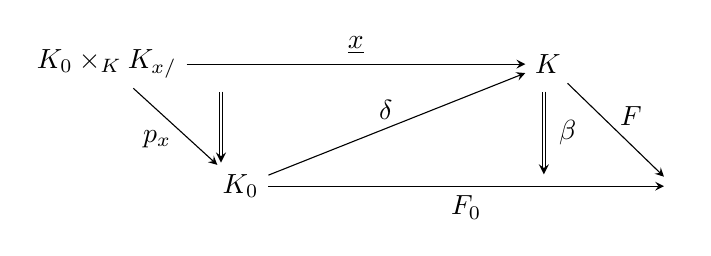
\begin{tikzpicture}[>=stealth]
\node (A) at (0,1.55) {$K_0\times_K K_{x/}$};
\node (K) at (5.6,1.55) {$K$};
\node (K0) at (1.7,0) {$K_0$};
\node (CC) at (7.2,0) {$\cC$};
\draw[->] (A) -- (K) node[midway,above] {$\underline{x}$};
\draw[->] (A) -- (K0) node[midway,below left=-2pt] {$p_x$};
\draw[->] (K0) -- (K) node[midway,above left=-2pt] {$\delta$};
\draw[->] (K0) -- (CC) node[midway,below] {$F_0$};
\draw[->] (K) -- (CC) node[midway,above right=-2pt] {$F$};
\draw[double,->] (1.45,1.2) -- (1.45,0.3);
\draw[double,->] (5.55,1.2) -- (5.55,0.15) node[midway,right=2pt] {$\beta$};
\end{tikzpicture}
\end{center}
与 $\beta$ 复合，得到自然变换 $F(x)\to F_0\circ p_x$；按定义，它对应于 $F(x)$ 沿
\[
\cC^{/F_0\circ p_x}\to\cC
\]
的一个提升，其中源 $\cC^{/F_0\circ p_x}$ 是第 6 讲第 5 节中的另一种切片范畴。现在命题断言：上述提升对任意 $x\in K$ 都是终对象（假定存在），当且仅当 $\beta$ 展示 $F$ 为 $F_0$ 沿 $\delta$ 的右 Kan 扩张。
\end{remark}

\begin{exercise}\label{L9-1.13}
对 $\pi\colon K\to\Delta^0$，证明 $\mathrm{RKE}_\pi u$ 存在当且仅当 $\lim u$ 存在。此外还有
\[
(\mathrm{RKE}_\pi u)(\ast)\simeq\lim u.
\]
如何找出 $(\mathrm{RKE}_\pi u)(\ast)$ 在 $\cC_{/u}$ 中的典范提升？
\end{exercise}

\begin{warning}\label{L9-1.14}
注意，纤维积 $K_0\times_K K_{x/}$ 也出现在 Quillen 定理 A 的陈述中。该定理断言下述两个条件等价：
\begin{enumerate}[label=(\roman*),leftmargin=2.6em,itemsep=0.1em]
\item 态射 $K_0\to K$ 是终的。
\item 对任意 $x\in K$，纤维积 $K_0\times_K K_{x/}$ 弱可缩。
\end{enumerate}
但请注意：(i) 与余极限因而与左 Kan 扩张有关，而定理~\ref{L9-1.8} 与右 Kan 扩张有关。我不知道如何联系这两个结果。
\end{warning}

\begin{exercise}\label{L9-1.15}
证明：右 Kan 扩张 $\mathrm{RKE}_\delta F_0$ 是点态的，当且仅当它被任意可表函子 $\operatorname{Maps}_{\cC}(c,-)\colon\cC\to\Grpd_\infty$ 保持。
\end{exercise}

\begin{proposition}\label{L9-1.16}
设 $\iota\colon K_0\to K$ 是 $\infty$-范畴之间的全忠实函子，$F_0\colon K_0\to\cC$ 是任意函子。假设点态右 Kan 扩张 $\mathrm{RKE}_\iota F_0$ 存在\footnote{这是指该右 Kan 扩张存在并且是点态的。}，则典范自然变换
\[
(\mathrm{RKE}_\iota F_0)\circ\iota\to F_0
\]
可逆。
\end{proposition}

\begin{proof}[证明梗概]
我们只需对任意 $x_0\in K_0$ 与 $x\coloneqq\iota(x_0)$，证明求值态射
\[
\lim_{K_0\times_K K_{x/}}(F_0\circ p_x)\to F_0(x_0)
\]
可逆。而这只需证明 $(x_0,\ x\xrightarrow{=}\iota(x_0))\in K_0\times_K K_{x/}$ 是始对象。这由显然的等价 $(K_0)_{x_0/}\to K_0\times_K K_{x/}$ 推出。
\end{proof}

\begin{exercise}\label{L9-1.17}
对 $\infty$-范畴 $K$，考虑显然的嵌入 $\iota\colon K\to K^{\triangleleft}$。证明：点态右 Kan 扩张 $\mathrm{RKE}_\iota u$ 存在，当且仅当 $u\colon K\to\cC$ 的极限存在。此外，$\mathrm{RKE}_\iota u$ 是延拓 $u$ 的极限图。
\end{exercise}

\begin{exercise}\label{L9-1.18}
证明：任意函子沿 $K^{\triangleleft}\to\Delta^0$ 的点态右 Kan 扩张总存在，且由在该函子于顶元 $\ast\in K^{\triangleleft}$ 处的取值给出。
\end{exercise}

\section{极限与极限交换}

\nitem\label{L9-2.1} 从现在起，$u\colon K_1\times K_2\to\cC$ 是 $\infty$-范畴之间的函子\footnote{事实上，这些结果可以推广到 $K_1$ 与 $K_2$ 是单纯集的情形。不过需要稍作修改构造与陈述。例子见 HTT.5.5.2.3。}。设 $\mathrm{pr}_i\colon K_1\times K_2\to K_i$ 与 $\pi_i\colon K_i\to[0]$ 是投影。

\begin{exercise}\label{L9-2.2}
点态右 Kan 扩张 $\mathrm{RKE}_{\mathrm{pr}_1}u$ 存在，当且仅当对任意 $x\in K_1$，$\lim_{K_2}u(x,-)$ 存在。此外，对任意 $x$，有典范同构
\[
(\mathrm{RKE}_{\mathrm{pr}_1}u)(x)\simeq\lim_{K_2}u(x,-).
\]
\end{exercise}

\nitem\label{L9-2.3} 作为推论，我们得到前几讲所承诺的构造
\[
K_1\to\cC,\qquad x\mapsto\lim_{K_2}u(x,-).
\]
结合命题~\ref{L9-1.6}，便得到\textbf{极限的分配律}。

\yizhu{“极限的分配律”指 $\lim_{K_1\times K_2}u\simeq\lim_{x\in K_1}\lim_{K_2}u(x,-)$，即乘积指标上的极限可以逐个因子计算（见推论~\ref{L9-2.4}）。此处的“分配”只是与环的分配律形式相仿，并非同一概念。\textbf{[来源：I]}}

\begin{corollary}\label{L9-2.4}
假设对任意 $x\in K_1$，$\lim_{K_2}u(x,-)$ 存在。则有典范同构
\[
\lim_{K_1\times K_2}u\xrightarrow{\ \simeq\ }\lim_{x\in K_1}\lim_{K_2}u(x,-).
\]
其中源存在当且仅当靶存在。
\end{corollary}

\begin{corollary}\label{L9-2.5}
假设：
\begin{itemize}[leftmargin=2.2em,itemsep=0.1em]
\item 对任意 $x\in K_1$，$\lim_{K_2}u(x,-)$ 存在；
\item 对任意 $y\in K_2$，$\lim_{K_1}u(-,y)$ 存在。
\end{itemize}
则有典范同构
\[
\lim_{x\in K_1}\lim_{K_2}u(x,-)\simeq\lim_{y\in K_2}\lim_{K_1}u(-,y).
\]
其中左端存在当且仅当右端存在。
\end{corollary}

\nitem\label{L9-2.6} 作为应用，我们得到下述关于 $\infty$-范畴的极限的结果。

\begin{theorem}\label{L9-2.7}
设 $u\colon K\to\Cat_\infty$，$i\mapsto\cC_i$，是 $\infty$-范畴的图。考虑求值函子
\[
\mathrm{ev}_i\colon\lim_{i\in K}\cC_i\to\cC_i.
\]
则有 $\infty$-群胚之间的典范等价
\begin{equation}\label{L9-eq2.1}
\operatorname{Maps}_{\lim_{i\in K}\cC_i}(x,y)\xrightarrow{\ \simeq\ }\lim_{i\in K}\operatorname{Maps}_{\cC_i}(\mathrm{ev}_i(x),\mathrm{ev}_i(y)).
\end{equation}
\end{theorem}

\begin{proof}[证明梗概]
按定义，
\[
\operatorname{Maps}_{\cC}(x,y)\simeq\{x\}\times_{\Fun(\{0\},\cC)}\Fun(\Delta^1,\cC)\times_{\Fun(\{1\},\cC)}\{y\}
\]
可以写成极限。于是定理由推论~\ref{L9-2.5} 以及 $\Fun(J,-)$ 保持极限这一事实推出。
\end{proof}

\begin{remark}\label{L9-2.8}
注意我们还有
\begin{equation}\label{L9-eq2.2}
\left(\lim_{i\in K}\cC_i\right)^{\simeq}\xrightarrow{\ \simeq\ }\lim_{i\in K}\cC_i^{\simeq},
\end{equation}
因为取核心是右伴随。实践中，关于 $\lim_{i\in K}\cC_i$ 的绝大多数（如果不是全部）结果都是用 \eqref{L9-eq2.1} 与 \eqref{L9-eq2.2} 证明的。
\end{remark}

\yizhu{“核心”即 $\infty$-范畴的 $\simeq$-群胚 $(-)^{\simeq}$，由把每个态射都视为可逆得到；勿与 t-结构的心（heart）相混。\textbf{[来源：B]}}

\section{如何使极限与余极限交换？}

\nitem\label{L9-3.1} 为简便起见，假设 $\cC$ 允许 $K_1$-指标的极限与 $K_2$-指标的余极限。特别地，练习~\ref{L9-2.2} 及其对偶蕴含下面所有的 LKE 与 RKE 都存在。

\begin{construction}\label{L9-3.2}
我们有一个显然的交换图
\begin{center}
\begin{tikzcd}[column sep=5.2em,row sep=3.4em]
\Fun(K_1\times K_2,\cC) & \Fun(K_1,\cC) \arrow[l, "-\circ \mathrm{pr}_1"] \\
\Fun(K_2,\cC) \arrow[u, "-\circ \mathrm{pr}_2"] & \Fun([0],\cC) \arrow[l, "-\circ \pi_2"] \arrow[u, "-\circ \pi_1"]
\end{tikzcd}
\end{center}
\end{construction}

与经典范畴论一样，我们可以沿水平方向取左伴随，得到一个自然变换\footnote{我们将在以后的讲中详细解释这一点。}
\begin{equation}\label{L9-eq3.1}
\begin{tikzcd}[column sep=5.2em,row sep=3.4em]
\Fun(K_1\times K_2,\cC) \arrow[rr, "\mathrm{LKE}_{\mathrm{pr}_1}"] \arrow[Rightarrow, from=1-1, to=2-3, shorten <=1.2em, shorten >=1.6em] & & \Fun(K_1,\cC) \\
\Fun(K_2,\cC) \arrow[u, "-\circ \mathrm{pr}_2"] \arrow[rr, "\mathrm{LKE}_{\pi_2}"] & & \Fun([0],\cC) \arrow[u, "-\circ \pi_1"]
\end{tikzcd}
\end{equation}

\begin{lemma}\label{L9-3.3}
自然变换 \eqref{L9-eq3.1} 可逆。
\end{lemma}

\begin{proof}[证明梗概]
设 $x\in K_1$ 是对象，$v\in\Fun(K_2,\cC)$ 是图。我们需要证明
\[
\mathrm{LKE}_{\mathrm{pr}_1}(v\circ\mathrm{pr}_2)(x)\to\mathrm{LKE}_{\pi_2}v(\pi_1(x))
\]
可逆。该态射可以等同于
\[
\colim_{(K_1)_{/x}\times_{K_1}(K_1\times K_2)}v'\to\colim_{K_2}v,
\]
其中 $v'$ 是复合 $(K_1)_{/x}\times_{K_1}(K_1\times K_2)\to K_2\xrightarrow{v}\cC$。因此我们只需证明态射 $(K_1)_{/x}\times_{K_1}(K_1\times K_2)\to K_2$ 是终的，这由 [第 7 讲，命题 3.15] 推出。
\end{proof}

\begin{construction}\label{L9-3.4}
由上述引理，我们有交换图
\begin{center}
\begin{tikzcd}[column sep=5.2em,row sep=3.4em]
\Fun(K_1\times K_2,\cC) \arrow[rr, "\mathrm{LKE}_{\mathrm{pr}_1}"] & & \Fun(K_1,\cC) \\
\Fun(K_2,\cC) \arrow[u, "-\circ \mathrm{pr}_2"] \arrow[rr, "\mathrm{LKE}_{\pi_2}"] & & \Fun([0],\cC) \arrow[u, "-\circ \pi_1"]
\end{tikzcd}
\end{center}
然后可以沿竖直方向取右伴随，得到自然变换
\begin{equation}\label{L9-eq3.2}
\begin{tikzcd}[column sep=5.2em,row sep=3.4em]
\Fun(K_1\times K_2,\cC) \arrow[rr, "\mathrm{LKE}_{\mathrm{pr}_1}"] \arrow[dd, "\mathrm{RKE}_{\mathrm{pr}_2}"'] & & \Fun(K_1,\cC) \arrow[dd, "\mathrm{RKE}_{\pi_1}"] \\
& & \\
\Fun(K_2,\cC) \arrow[rr, "\mathrm{LKE}_{\pi_2}"] \arrow[Rightarrow, from=3-1, to=1-3, "{\alpha}"', shorten <=1.4em, shorten >=1.6em] & & \Fun([0],\cC)
\end{tikzcd}
\end{equation}
特别地，对任意 $u\colon K_1\times K_2\to\cC$，我们得到典范态射
\[
\colim_{y\in K_2}\lim_{K_1}u(-,y)\to\lim_{x\in K_1}\colim_{K_2}u(x,-).
\]
\end{construction}

\begin{definition}\label{L9-3.5}
若 \eqref{L9-eq3.2} 可逆，则称 $\cC$ 中 $K_1$-指标的极限与 $K_2$-指标的余极限\textbf{交换}。
\end{definition}

\nitem\label{L9-3.6} 下一讲我们将解释下述结果。

\begin{theorem}\label{L9-3.7}
在 $\Grpd_\infty$ 中，滤过余极限与有限极限交换。
\end{theorem}

\begin{remark}\label{L9-3.8}
一旦引入了紧生成的 $\infty$-范畴，就容易推出上述定理在任何这样的 $\infty$-范畴中成立。
\end{remark}

\begin{warning}\label{L9-3.9}
滤过或有限指标 $\infty$-范畴的定义是微妙的。例如，有限的普通范畴可能不是有限的 $\infty$-范畴。
\end{warning}

\begin{theorem}\label{L9-3.10}
在 $\Grpd_\infty$ 中，筛余极限与有限积交换。
\end{theorem}

\begin{theorem}\label{L9-3.11}
在 $\Grpd_\infty$ 中，小余极限被基变换保持。
\end{theorem}

\appendixsection{图的分解}

\begin{exercise}\label{L9-A.1}
设 $K$ 是单纯集，$K_1,K_2\subset K$ 是 $K$ 的单纯子集，使得
\[
K_1\sqcup_{K_1\cap K_2}K_2\to K
\]
是同构。设 $u\colon K\to\cC$ 是 $\infty$-范畴中的图。证明有典范同构
\[
\lim_K u\xrightarrow{\ \simeq\ }\lim_{K_1}u\times_{\lim_{K_1\cap K_2}u}\lim_{K_2}u.
\]
其中若靶存在，则源存在。
\end{exercise}

\begin{exercise}\label{L9-A.2}
证明 $x\rightrightarrows y$ 的等化子同构于 $x\times_{x\times y}x$。
\end{exercise}

\begin{exercise}\label{L9-A.3}
设 $K$ 是单纯集，$\mathrm{Sub}(K)$ 是 $K$ 的单纯子集构成的部分序集，视为普通范畴。设 $I\to\mathrm{Sub}(K)$，$i\mapsto K_i$ 是普通范畴之间的函子。求一个充分条件，使得对任意图 $u\colon K\to\cC$，都有典范同构
\[
\lim_K u\xrightarrow{\ \simeq\ }\lim_{i\in I}\lim_{K_i}u.
\]
\end{exercise}

\nitem\label{L9-A.4} \textbf{建议阅读}\quad HTT.4.2.3, Ker.03CY.
